\documentclass[aspectratio=169,9pt]{beamer}
\usepackage{amsmath,amssymb}
\usepackage{graphicx}
\usepackage{booktabs}

\usetheme{default}
\setbeamertemplate{navigation symbols}{}
\setbeamertemplate{footline}[frame number]
\setbeamerfont{frametitle}{size=\large,series=\bfseries}
\setbeamertemplate{itemize items}[circle]
\setlength{\leftmargini}{1.2em}

% figures are written by the pipeline to outputs/
\graphicspath{{../outputs/}{outputs/}}
\newcommand{\given}{\,|\,}
\newcommand{\bin}{\operatorname{binomial}}
\newcommand{\dnew}{\Delta D^{\mathrm{new}}}
\newcommand{\dold}{\Delta D^{\mathrm{old}}}

% The numbers on the slides "The two delays are not independent" and "Early
% results" are typed in by hand, from the reports and from the run
% runs/2026-10-13_12_06_deaths_bring_reports on the branch experiment-results.
% They are not yet written by the pipeline.

\begin{document}

% ---------------------------------------------------------------------------
\begin{frame}{Bundibugyo virus disease, 2026: joint modelling of cases, deaths and the case fatality ratio}
\centering
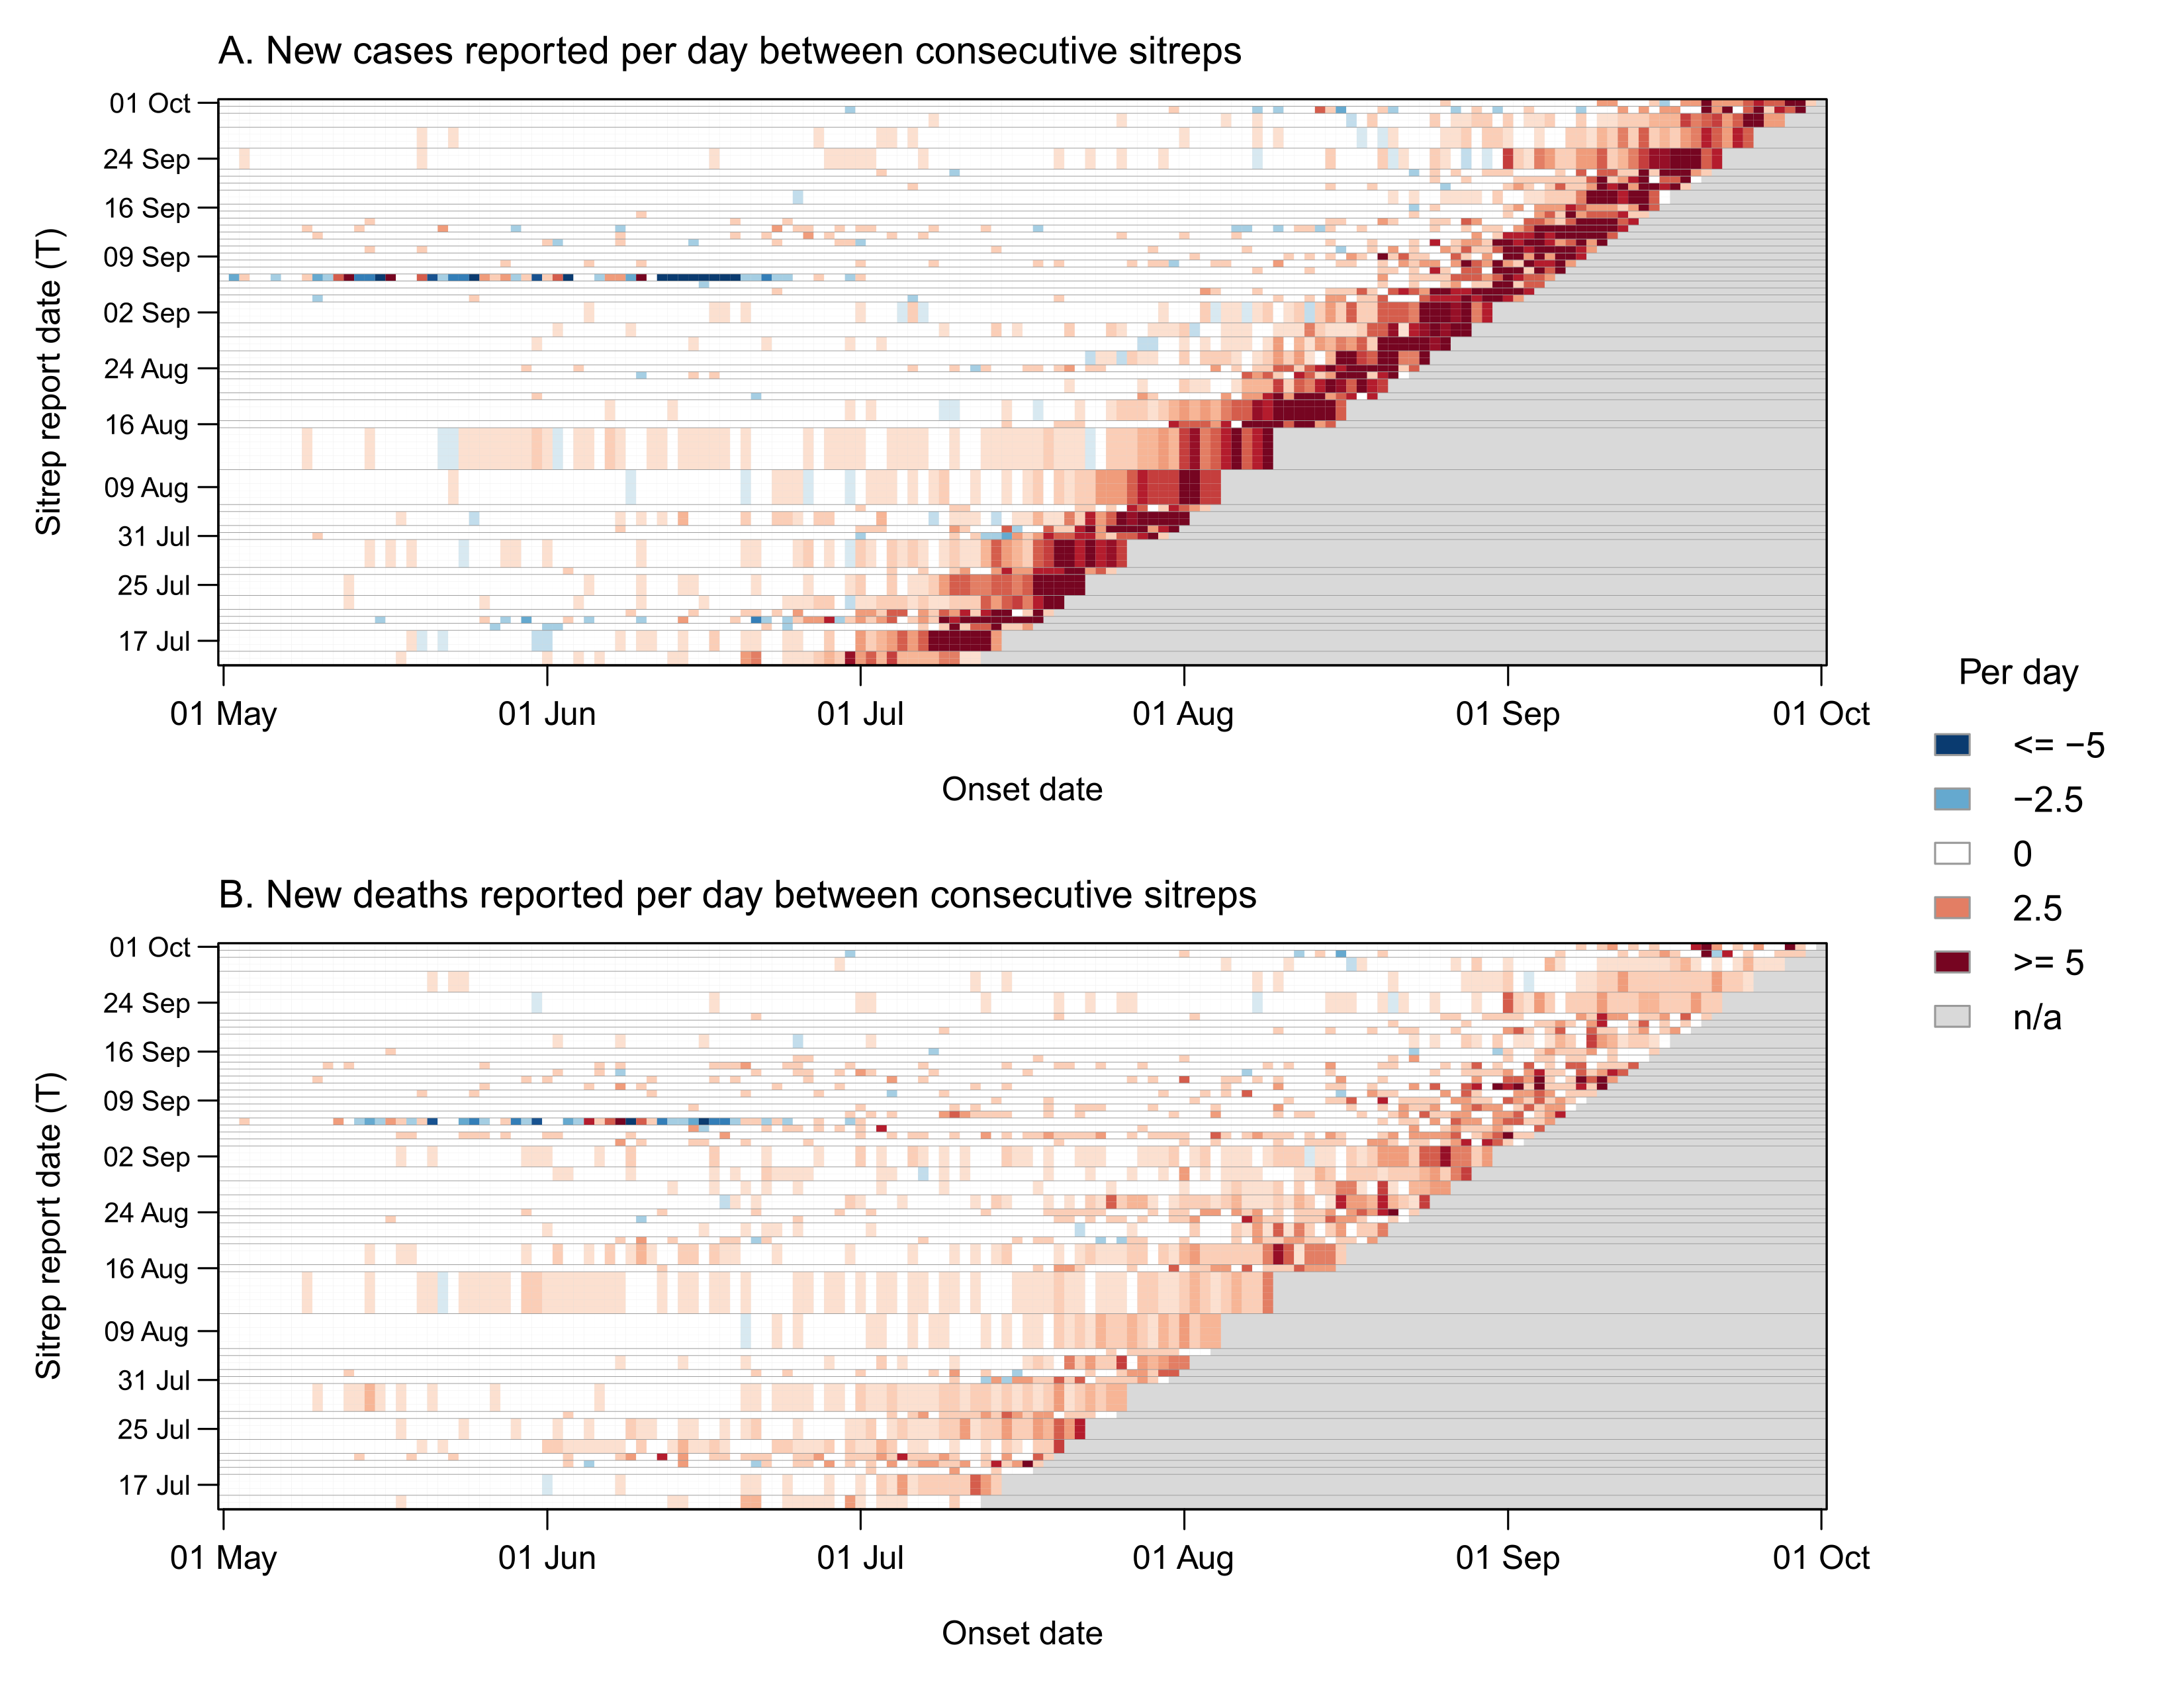
\includegraphics[height=0.76\textheight]{New cases and deaths with onset between consecutive sitreps.png}

\smallskip
{\small Each situation report revises the counts of cases and of deaths for
every onset date. Deaths go on being added for much longer than cases.}
\end{frame}

% ---------------------------------------------------------------------------
\begin{frame}{What the reports show}
Each report gives an epidemic curve by date of onset, with each day's cases
split into alive and dead. For onset day $t$ and a report made on day $t_j$:
\begin{align*}
C(t\given t_j) &: \text{confirmed cases counted for day $t$};\\
D(t\given t_j) &: \text{the number of those cases shown as dead},\quad D\le C.
\end{align*}

\begin{itemize}
\item \textbf{No dates of death.} A death is counted on the onset day of its
case. We see only that the count of dead for a day rose between two reports.
\item \textbf{The dead are among the cases already counted.} A death cannot
be shown before its case is in the report.
\item \textbf{Deaths lag cases.} At 7 to 14 days after onset the case count
is about 79\% of its latest value and the death count about 60\%.
\end{itemize}

\bigskip
So the crude ratio $D/C$ is too low for recent onset days: 0.45 to 0.49 for
onset fortnights up to early September, 0.28 for the latest fortnight.
\end{frame}

% ---------------------------------------------------------------------------
\begin{frame}{Approach}
Unknown for each onset day: the true cases $I(t)$ and, of those, the cases
which will die, $F(t)$. We model how both arise and how they come to be
shown in the reports:
\[
p\bigl(I, F, R, c, \theta, \phi \given C, D\bigr)\;\propto\;
\underbrace{p\bigl(C, D\given I, F, \theta, \phi\bigr)}_{\text{reporting}}\;
\underbrace{p\bigl(F\given I, c\bigr)}_{\text{fatality}}\;
\underbrace{p\bigl(I\given R\bigr)}_{\text{transmission}}\;
p(R)\,p(c)\,p(\theta)\,p(\phi)
\]

\bigskip
\begin{itemize}
\item $R$: reproduction numbers $R_t$. $c$: case fatality ratios $c_t$, by
onset day.
\item $\theta$: reporting of cases. $\phi$: recording of deaths.
\item $R_t$, $c_t$ and both delays can change at unknown times.
\end{itemize}

\bigskip
The aims are the eventual numbers of cases and of deaths for recent onset
days, and a case fatality ratio which allows for deaths not yet recorded.
\end{frame}

% ---------------------------------------------------------------------------
\begin{frame}{Starting point: the model of cases}
\textbf{Transmission.} A renewal process with overdispersion; $R_t$
piecewise constant, with changes at unknown times:
\[
I(t)\sim\operatorname{NB}\bigl(R_t\,\Lambda_t,\ \kappa\bigr),\qquad
\Lambda_t=\sum_{s=1}^{40}\omega_s\,I(t-s)
\]

\textbf{Reporting.} Each case is reported after a gamma$(\mu,\sigma)$ delay
from onset, with each day's hazard multiplied by an effect of the day of the
week. $S^{C}(t\given t')$: probability a case with onset on day $t$ is not
yet reported at $t'$. Between reports $t_{j-1}$ and $t_j$:
\[
\Delta C(t\given t_j)\sim\bin\Bigl(I(t)-C(t\given t_{j-1}),\
1-\frac{S^{C}(t\given t_j)}{S^{C}(t\given t_{j-1})}\Bigr)
\]

\textbf{Wrong records.} Records are added in error in proportion to
reporting activity (rate $\eta$) and each is later removed with probability
$\rho$ a day. Summed out exactly by a forward recursion.

\bigskip
\textbf{Changes at unknown times.} $R_t$ and $(\mu,\sigma)$ are constant
within segments; each day starts a new segment with probability $p$,
$p\sim\operatorname{beta}(1,T)$.
\end{frame}

% ---------------------------------------------------------------------------
\begin{frame}{Fatal cases, and two delays for each}
Of the $I(t)$ cases with onset on day $t$, $F(t)$ will die and
$N(t)=I(t)-F(t)$ will not:
\[
F(t)\sim\bin\bigl(I(t),\ c_t\bigr)
\]

\medskip
Each fatal case has two delays from onset:

\smallskip
\begin{center}
\renewcommand{\arraystretch}{1.3}
\begin{tabular}{lll}
\toprule
 & Delay & Probability it has not happened by $t'$ \\
\midrule
The case is reported & $X\sim\text{gamma}(\mu,\sigma)$ & $S^{C}(t\given t')$ \\
The death is recorded & $Y\sim\text{gamma}(\mu^{d},\sigma^{d})$ & $S^{D}(t\given t')$ \\
\bottomrule
\end{tabular}
\end{center}

\medskip
\begin{itemize}
\item $Y$ is the time from onset to death plus the time for the death to be
entered in the records. The two parts are not separated.
\item A fatal case is \textbf{shown as dead} at $t'$ once it is reported
\emph{and} its death is recorded: $\max(X,Y)\le t'-t$.
\item Reported but death not yet recorded ($X\le t'-t<Y$): shown as alive.
\item Each delay has its own effects of the day of the week.
\end{itemize}
\end{frame}

% ---------------------------------------------------------------------------
\begin{frame}{What a report shows}
The cases of onset day $t$ in the report of $t_j$ are of three kinds:

\medskip
\begin{center}
\renewcommand{\arraystretch}{1.4}
\begin{tabular}{lll}
\toprule
 & Number & Shown as \\
\midrule
Non-fatal cases reported so far & $C^{N}(t\given t_j)$ & alive \\
Fatal cases reported, death not yet recorded & $C^{F}(t\given t_j)-D(t\given t_j)$ & alive \\
Fatal cases reported, death recorded & $D(t\given t_j)$ & dead \\
\bottomrule
\end{tabular}
\end{center}

\bigskip
\begin{itemize}
\item Observed: $C=C^{N}+C^{F}$ and $D$.
\item Not observed: the split of $C$ into $C^{F}$ and $C^{N}$. Some of the
cases shown as alive will die.
\item So for each onset day there is one unobserved path over reports,
$C^{F}(t\given t_1),\,C^{F}(t\given t_2),\dots$
\end{itemize}
\end{frame}

% ---------------------------------------------------------------------------
\begin{frame}{From one report to the next}
With $p^{F},p^{N}$ the probabilities that a fatal or non-fatal case not
reported by $t_{j-1}$ is reported by $t_j$:

\smallskip
\begin{align*}
\text{fatal cases new to the report}\quad
 & \Delta C^{F}(t\given t_j)\sim\bin\bigl(F(t)-C^{F}(t\given t_{j-1}),\ p^{F}(t\given t_j)\bigr)\\[3pt]
\text{non-fatal cases new to the report}\quad
 & \Delta C^{N}(t\given t_j)\sim\bin\bigl(N(t)-C^{N}(t\given t_{j-1}),\ p^{N}(t\given t_j)\bigr)\\[3pt]
\text{new cases already shown as dead}\quad
 & \dnew(t\given t_j)\sim\bin\bigl(\Delta C^{F}(t\given t_j),\ g(t\given t_j)\bigr)\\[3pt]
\text{cases shown as alive before, now dead}\quad
 & \dold(t\given t_j)\sim\bin\Bigl(C^{F}(t\given t_{j-1})-D(t\given t_{j-1}),\
 1-\frac{S^{D}(t\given t_j)}{S^{D}(t\given t_{j-1})}\Bigr)
\end{align*}

\smallskip
Observed: $\Delta C=\Delta C^{F}+\Delta C^{N}$ and $\Delta D=\dnew+\dold$.

\medskip
\small
\begin{itemize}
\item If $X$ and $Y$ are independent, $p^{F}=p^{N}$ and
$g(t\given t_j)=1-S^{D}(t\given t_j)$: being unreported until now says
nothing about whether the death has been recorded.
\item Example: 10 cases, 3 dead, then 12 cases, 5 dead. The 2 new deaths may
be among the 7 shown as alive before, or the 2 new cases, or one of each.
The likelihood sums over these.
\item Given $I(t)$ and $F(t)$, each onset day is a hidden Markov chain over
reports with state $C^{F}$.
\end{itemize}
\end{frame}

% ---------------------------------------------------------------------------
\begin{frame}{The two delays are not independent}
Under independence, among the reported cases of an onset day the share
shown as dead at time $u$ since onset is
\[
c_t\,\bigl[1-S^{D}(u)\bigr],
\]
which starts near zero and can only rise. The reports do not look like this
(onset days 12 July to 5 September):

\begin{columns}[c]
\begin{column}{0.4\textwidth}
\centering
\renewcommand{\arraystretch}{1.25}
\begin{tabular}{lc}
\toprule
Time since onset & Share shown as dead \\
\midrule
0 to 1 days & 0.43 \\
About a week & 0.34 \\
2 to 3 months & 0.46 \\
\bottomrule
\end{tabular}
\end{column}
\begin{column}{0.55\textwidth}
\begin{itemize}
\item Cases reported soon after onset are already dead as often as cases
followed for months.
\item To fit this the independent model needs a delay to death with a spike
near zero and a very long tail: gamma shape about 0.2, mean 46 days, sd 97.
\item It then expects many deaths still to come, and overshoots: for onset
days to 5 September, about 3{,}100 deaths against 2{,}502 recorded by
1 October.
\end{itemize}
\end{column}
\end{columns}

\bigskip
Many fatal cases, it seems, enter the records \emph{because} they have died.
\end{frame}

% ---------------------------------------------------------------------------
\begin{frame}{A death which brings about the report}
A proportion $\tau$ of fatal cases are reported when their death is recorded,
if they have not been reported by then:
\[
\text{time to being reported}=
\begin{cases}
\min(X,Y) & \text{with probability } \tau\\
X & \text{with probability } 1-\tau
\end{cases}
\qquad\text{shown as dead from } Y \text{ or } \max(X,Y) \text{ respectively.}
\]

A fatal case is not yet reported at $t'$ with probability
\[
M(t\given t')=S^{C}(t\given t')\,\bigl[(1-\tau)+\tau\,S^{D}(t\given t')\bigr],
\qquad
p^{F}(t\given t_j)=1-\frac{M(t\given t_j)}{M(t\given t_{j-1})}.
\]

A fatal case new to the report of $t_j$ is shown as alive only if it was
reported through $X$ and its death is not yet recorded, whichever kind it
is. So
\[
g(t\given t_j)=1-\frac{\bigl[S^{C}(t\given t_{j-1})-S^{C}(t\given t_j)\bigr]\,S^{D}(t\given t_j)}
       {M(t\given t_{j-1})-M(t\given t_j)}.
\]

\small
\begin{itemize}
\item Only $p^{F}$ and $g$ change. The probability for $\dold$ is as before:
a case shown as alive has yet to have its death recorded.
\item $\tau=0$ is the independent model. $\tau\sim\operatorname{beta}(1,1)$.
\end{itemize}
\end{frame}

% ---------------------------------------------------------------------------
\begin{frame}{What this changes}
\begin{itemize}
\item \textbf{Fatal cases are reported sooner than others,} and the cases
reported early are more often fatal than those reported later.
\item \textbf{The share shown as dead can start high, fall and rise again:}
high among the first cases reported, lower as other cases are reported,
higher again as the slower deaths are recorded.
\item \textbf{$\tau=1$ does not mean every fatal case first appears dead.}
Each fatal case is then a race between its report and its death being
recorded; it means only that a recorded death is never left without its
case.
\item \textbf{The delay to death no longer has to explain early deaths,} so
it is free to match how long deaths go on being recorded.
\end{itemize}

\bigskip
One parameter is added, and the likelihood is still exact: the hidden state
for each onset day is unchanged.

\bigskip
{\small Not used alongside this: a separate reporting delay for fatal cases
(a rescaling $e^{\nu}$ of time). Both let fatal cases be reported sooner,
and the reports are unlikely to tell them apart.}
\end{frame}

% ---------------------------------------------------------------------------
\begin{frame}{Wrong records, now alive or dead}
Counts of deaths also fall now and then (18 times in 2{,}129 comparisons
of consecutive reports, never by more than 2; on 11 of these the case
count fell too).

\bigskip
As before, wrong records are added in proportion to reporting activity and
removed at rate $\rho$ a day. Each new wrong record is shown as dead with
probability $\delta$:
\[
C(t\given t_j)=C^{N}+C^{F}+E^{A}+E^{D},
\qquad
D(t\given t_j)=D^{G}+E^{D},
\]
with $E^{A},E^{D}$ the wrong records shown as alive and as dead, and $D^{G}$
the genuine fatal cases shown as dead.

\bigskip
\begin{itemize}
\item The hidden state for each onset day becomes
$(C^{F},E^{A},E^{D})$, with $E^{A}+E^{D}$ limited to a small number.
\item A fall in deaths with no fall in cases needs nothing further: a wrong
record shown as dead is removed while a genuine case is added.
\item $\delta\sim\operatorname{beta}(1,1)$.
\end{itemize}
\end{frame}

% ---------------------------------------------------------------------------
\begin{frame}{Changes at unknown times}
Four quantities are piecewise constant in the onset day, each with its own
change points and the same prior on them (each day starts a new segment
with probability $p$, $p\sim\operatorname{beta}(1,T)$).

\bigskip
\begin{center}
\renewcommand{\arraystretch}{1.35}
\begin{tabular}{lll}
\toprule
Quantity & Prior within a segment & Minimum segment \\
\midrule
$R_t$ & gamma & 7 days \\
Reporting delay $(\mu,\sigma)$ & hierarchical log-normal & 14 days \\
Case fatality ratio $c_t$ & $\operatorname{beta}(1,1)$ & 14 days \\
Delay to death recorded $(\mu^{d},\sigma^{d})$ & hierarchical log-normal & 14 days \\
\bottomrule
\end{tabular}
\end{center}

\bigskip
\begin{itemize}
\item $c_t$ is indexed by onset day: a change is a change between cohorts of
cases by when they fell ill.
\item Hierarchical: the segments of a delay are log-normal about a common
centre, which has its own prior.
\item An alternative for the delay to death, not shown here: a random walk
from week to week on the log scale.
\end{itemize}
\end{frame}

% ---------------------------------------------------------------------------
\begin{frame}{Fitting}
Metropolis within Gibbs, extending the sampler for cases.

\bigskip
\begin{itemize}
\item \textbf{$F(t)$, with the path summed out.} Forward filtering over the
reports of an onset day gives $p(\text{reports}\given I(t),F(t))$; a small
change in $F(t)$ is proposed and accepted by Metropolis.
\item \textbf{Paths $(C^{F},E^{A},E^{D})$.} Drawn exactly by backward
sampling. The state space is small: $C^{F}$ can rise between two reports by
no more than the case count does.
\item \textbf{$I(t)$ and $F(t)$ given the paths.} $I(t)$ from its discrete
conditional with $F(t)$ summed out, then $F(t)$ given $I(t)$.
\item \textbf{$c_t$ segments.} Drawn exactly with segment values integrated
out (beta-binomial), as for $R_t$.
\item \textbf{Delay segments, for cases and for deaths.} Split, merge and
shift moves.
\item \textbf{$\tau$, $\rho$, effects of the day of the week.} Random-walk
Metropolis given the paths. $\delta$ and $\eta$ from their conjugate
conditionals.
\end{itemize}

\bigskip
{\small The first step is needed because, once every case of an onset day is
reported, $C^{F}=F(t)$ and neither can move with the other held fixed.}
\end{frame}

% ---------------------------------------------------------------------------
\begin{frame}{What can and cannot be learned}
\begin{itemize}
\item \textbf{A recent fall in $c_t$ and deaths not yet recorded look the
same.} For onset days in the last three to four weeks, $c_t$ rests mostly
on the delay to death estimated from earlier onset days.
\item \textbf{A change in the delay to death and a change in $c_t$ at about
the same time are hard to tell apart.}
\item \textbf{Old onset days say little about the reporting delay of cases,
but much about deaths.} Nearly all their cases are in the first report
which includes them; their deaths go on being recorded for weeks.
\item \textbf{Deaths inform recent case numbers a little:} many early deaths
among few reported cases make a small $I(t)$ unlikely.
\end{itemize}
\end{frame}

% ---------------------------------------------------------------------------
\begin{frame}{Early results: reports up to 5 September (chains not yet converged)}
\centering
\renewcommand{\arraystretch}{1.25}
\begin{tabular}{llccc}
\toprule
 & & \multicolumn{2}{c}{Recorded for the same onset days} & \\
\cmidrule(lr){3-4}
Onset days & & by 5 Sep (given to the fit) & by 1 Oct (hindsight) & Estimate \\
\midrule
All & Cases & 5{,}079 & 5{,}504 & 5{,}556 (5{,}485--5{,}622) \\
 & Deaths & 2{,}111 & 2{,}502 & 2{,}711 (2{,}631--2{,}812) \\
Latest 14 & Cases & 430 & 830 & 879 (815--940) \\
 & Deaths & 169 & 407 & 434 (397--476) \\
\bottomrule
\end{tabular}

\medskip
\begin{tabular}{lcc}
\toprule
 & Independent delays & A death can bring the report \\
\midrule
Deaths, all onset days & about 3{,}130 & 2{,}711 (2{,}631--2{,}812) \\
Mean delay to death recorded, latest onset days & about 45 days & 12 (10--14) days \\
Share $\tau$ & -- & 0.50 (0.33--0.64) \\
\bottomrule
\end{tabular}

\medskip
\begin{minipage}{0.9\textwidth}
\small Posterior medians and 90\% intervals; 4 chains of 800 iterations.
The counts recorded by 1 October are a lower bound for deaths, which are
still being added. $\hat{R}$ is at most 1.05 for the totals but 1.7 for the
sd of the delay to death and 1.3 for $\tau$, so these are provisional.
\end{minipage}
\end{frame}

% ---------------------------------------------------------------------------
\begin{frame}{Still to do}
\begin{itemize}
\item \textbf{Longer chains.} The totals agree between chains; the delay to
death and $\tau$ do not yet.
\item \textbf{Later analysis dates.} Fits to the reports up to 15 September
and 1 October overshoot deaths by more than the fit to 5 September.
\item \textbf{Early onset days.} For onsets in May the mean delay to death
is estimated at 40 to 60 days, against 10 to 12 from mid-August.
\item \textbf{Checks.} The share shown as dead by time since onset, from the
fitted model against the reports.
\item \textbf{Deaths counted on the day of death.} Some fatal cases with no
known onset date may be counted on the day they died. This is built, but
cannot yet be combined with a death which brings about the report.
\end{itemize}
\end{frame}

% ---------------------------------------------------------------------------
\begin{frame}
\centering
\Huge Any questions?
\end{frame}

% ---------------------------------------------------------------------------
\appendix

\begin{frame}{Appendix: onset days first seen late}
The first report is that of 12 July, and already shows cases with onset from
April. The analysis starts at the onset day of 11 May.

\bigskip
For an onset day before the first report, the first report $t_1$ which
includes it is treated as any other, with nothing reported before it:
\[
C^{F}(t\given t_1)\sim\bin\bigl(F(t),\ 1-M(t\given t_1)\bigr),\qquad
C^{N}(t\given t_1)\sim\bin\bigl(N(t),\ 1-S^{C}(t\given t_1)\bigr).
\]

\begin{itemize}
\item No change in the reporting delay of cases is allowed among these
days: they say almost nothing about it, so a segment there would be drawn
from its prior.
\item Changes in $c_t$ and in the delay to death are allowed on any day.
\end{itemize}
\end{frame}

% ---------------------------------------------------------------------------
\begin{frame}{Appendix: the report of 6 September}
This report corrected the records of onset days before 28 June: 137 records
removed, 48 added, and some records changed from dead to alive. The model
of wrong records (few, removed one at a time) cannot follow counts across
it.

\bigskip
\begin{itemize}
\item For the corrected onset days, the reports made before 6 September are
left out, and that report is treated as their first.
\item Those days are then 71 to 118 days old when first seen: nearly all
their cases are reported and deaths recorded, so $c_t$ is close to the
share shown as dead.
\item What is given up: the earlier reports showed the deaths of those days
being recorded over many weeks, so they now say little about the delay to
death in May and June.
\item The correction itself is not modelled.
\end{itemize}
\end{frame}

\end{document}
